\chapter{Motivations \& Evolution}
To do
\section{Motivations}

Social media has an important role in the real world and has an impact which was probably under
estimated a couple of years ago. Historical events like the arab spring or the election in Cambodia are two 
examples which show social media can be a powerful force for change when compared to other media. 
These events lead to studies about human behaviour and engagement on these platforms.\\
For users, one of the main goal is to increase the time efficiency on social media. Today, 27\% of an hour 
spent online is on social media. There are many methods used to try to make users' time on social media
more efficient.  As we saw with EdgeRank, the filtering of the information is one of the main ones. 

\begin{figure}[tb] 
\centering 
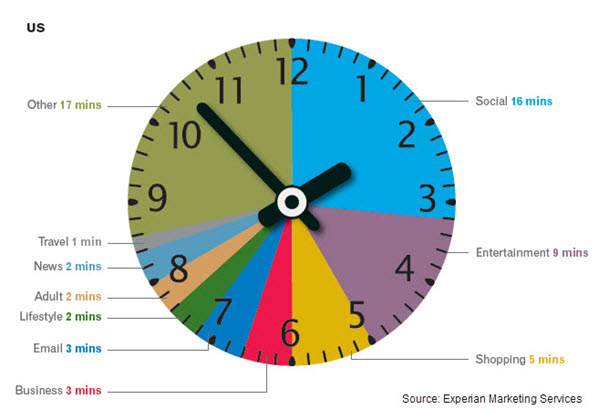
\includegraphics[width=0.5\columnwidth]{motiv/clock-time} 
\caption[A floating figure]{The clock shows the repartition of the web TO DO  \emph{Galleria di stampe}, of M.~Escher, got from \url{http://www.mcescher.com/}).}
\label{fig:clock} 
\end{figure}

Recently, Twitter had to deal with an engagement problem. As we can see on figure 1.2, despite is 550
million users, Twitter has an engagement lower than Facebook or Instagram: this weakness led to  a drop in
its stock price. However, "engagement" has no scientific definition and by consequence, there is no unique
solution to this problem. By considering a new design which reduce the overload of information, it will be
possible to analyse more details relating to the problem of engagement. By doing this it will be possible to
improve user time efficiency and twitter engagement issues.

\begin{figure}[tb] 
\centering 
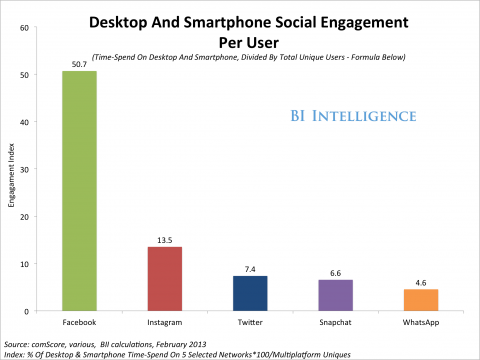
\includegraphics[width=0.5\columnwidth]{motiv/social-engag} 
\caption[A floating figure]{Social Engagement TO DO  \emph{Galleria di stampe}, of M.~Escher, got from \url{http://www.mcescher.com/}).}
\label{fig:engagement} 
\end{figure}

\section{Project evolution}

Information overload is a large topic and many aspects could have been approached. By viewing Figure 1.3 can understand better why it was decide to focus the research on Twitter. Our three main criteria are: privacy, 
content and technique. \\
Firstly, with Gmail, privacy and content were being dealt with. Due to the email variate and the personal 
characters of email, it was difficult to establish a protocol in order to improve the filtering of the emails.
Secondly, we started to develop, with a similar design, applications based on different social media like 
Reddit or Tumblr.\\
Finally, Tinder and Twitter were found to be of particular interest, due to the design of the Tinder app and the 
140 character limit of Twitter. For these two reasons and Twitter's simple API The idea of Twinder was arrived 
upon.\\
You can find in annex the diagram showing the evolution of the project through 3 aspects: technique, apps 
implementation and research.

\begin{figure}[tb] 
\centering 
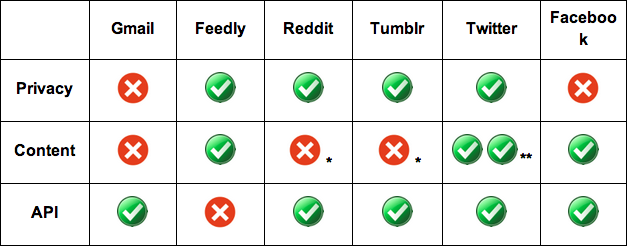
\includegraphics[width=0.5\columnwidth]{motiv/table_analysis} 
\caption[A floating figure]{Lalala TO DO  \emph{Galleria di stampe}, of M.~Escher, got from \url{http://www.mcescher.com/}).}
\label{fig:table_analysis} 
\end{figure}

 *:content is not constant
**: 140 char with image or not

x: problem for implementing the experiment
v: ok for implementing the experiment


